% Created by tikzDevice version 0.12.6 on 2024-01-31 20:03:03
% !TEX encoding = UTF-8 Unicode
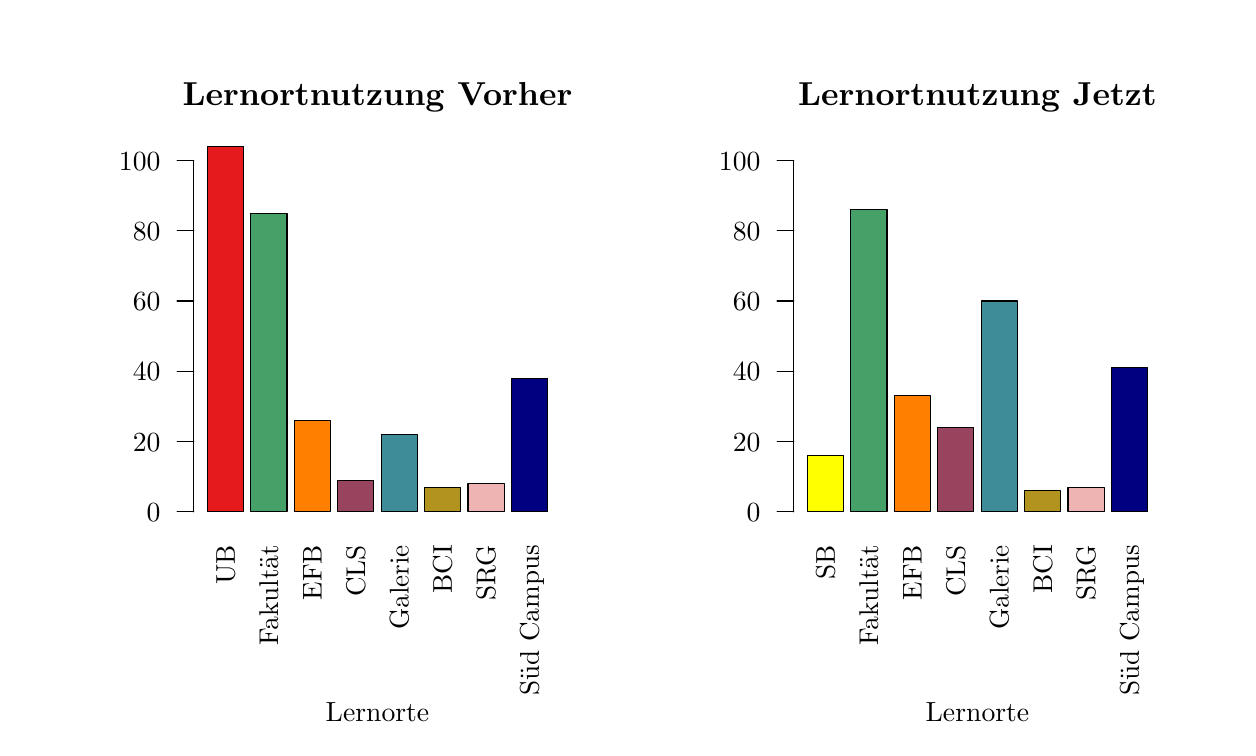
\begin{tikzpicture}[x=1pt,y=1pt]
\definecolor{fillColor}{RGB}{255,255,255}
\path[use as bounding box,fill=fillColor,fill opacity=0.00] (0,0) rectangle (433.62,252.94);
\begin{scope}
\path[clip] (  0.00,  0.00) rectangle (216.81,252.94);
\definecolor{drawColor}{RGB}{0,0,0}
\definecolor{fillColor}{RGB}{228,26,28}

\path[draw=drawColor,line width= 0.4pt,line join=round,line cap=round,fill=fillColor] ( 64.92, 78.00) rectangle ( 78.00,210.02);
\definecolor{fillColor}{RGB}{70,161,105}

\path[draw=drawColor,line width= 0.4pt,line join=round,line cap=round,fill=fillColor] ( 80.62, 78.00) rectangle ( 93.70,185.90);
\definecolor{fillColor}{RGB}{255,127,0}

\path[draw=drawColor,line width= 0.4pt,line join=round,line cap=round,fill=fillColor] ( 96.32, 78.00) rectangle (109.40,111.01);
\definecolor{fillColor}{RGB}{153,68,94}

\path[draw=drawColor,line width= 0.4pt,line join=round,line cap=round,fill=fillColor] (112.01, 78.00) rectangle (125.10, 89.43);
\definecolor{fillColor}{RGB}{61,140,152}

\path[draw=drawColor,line width= 0.4pt,line join=round,line cap=round,fill=fillColor] (127.71, 78.00) rectangle (140.80,105.93);
\definecolor{fillColor}{RGB}{178,147,31}

\path[draw=drawColor,line width= 0.4pt,line join=round,line cap=round,fill=fillColor] (143.41, 78.00) rectangle (156.49, 86.89);
\definecolor{fillColor}{RGB}{238,180,180}

\path[draw=drawColor,line width= 0.4pt,line join=round,line cap=round,fill=fillColor] (159.11, 78.00) rectangle (172.19, 88.16);
\definecolor{fillColor}{RGB}{0,0,128}

\path[draw=drawColor,line width= 0.4pt,line join=round,line cap=round,fill=fillColor] (174.81, 78.00) rectangle (187.89,126.24);
\end{scope}
\begin{scope}
\path[clip] (  0.00,  0.00) rectangle (433.62,252.94);
\definecolor{drawColor}{RGB}{0,0,0}

\node[text=drawColor,rotate= 90.00,anchor=base east,inner sep=0pt, outer sep=0pt, scale=  0.98] at ( 74.83, 66.00) {UB};

\node[text=drawColor,rotate= 90.00,anchor=base east,inner sep=0pt, outer sep=0pt, scale=  0.98] at ( 90.53, 66.00) {Fakultät};

\node[text=drawColor,rotate= 90.00,anchor=base east,inner sep=0pt, outer sep=0pt, scale=  0.98] at (106.23, 66.00) {EFB};

\node[text=drawColor,rotate= 90.00,anchor=base east,inner sep=0pt, outer sep=0pt, scale=  0.98] at (121.93, 66.00) {CLS};

\node[text=drawColor,rotate= 90.00,anchor=base east,inner sep=0pt, outer sep=0pt, scale=  0.98] at (137.63, 66.00) {Galerie};

\node[text=drawColor,rotate= 90.00,anchor=base east,inner sep=0pt, outer sep=0pt, scale=  0.98] at (153.33, 66.00) {BCI};

\node[text=drawColor,rotate= 90.00,anchor=base east,inner sep=0pt, outer sep=0pt, scale=  0.98] at (169.03, 66.00) {SRG};

\node[text=drawColor,rotate= 90.00,anchor=base east,inner sep=0pt, outer sep=0pt, scale=  0.98] at (184.72, 66.00) {Süd Campus};
\end{scope}
\begin{scope}
\path[clip] (  0.00,  0.00) rectangle (216.81,252.94);
\definecolor{drawColor}{RGB}{0,0,0}

\node[text=drawColor,anchor=base,inner sep=0pt, outer sep=0pt, scale=  1.20] at (126.41,224.80) {\bfseries Lernortnutzung Vorher};

\node[text=drawColor,anchor=base,inner sep=0pt, outer sep=0pt, scale=  1.00] at (126.41,  2.40) {Lernorte};

\node[text=drawColor,rotate= 90.00,anchor=base,inner sep=0pt, outer sep=0pt, scale=  1.00] at ( -8.40,141.47) {Anzahl};
\end{scope}
\begin{scope}
\path[clip] (  0.00,  0.00) rectangle (433.62,252.94);
\definecolor{drawColor}{RGB}{0,0,0}

\path[draw=drawColor,line width= 0.4pt,line join=round,line cap=round] ( 60.00, 78.00) -- ( 60.00,204.94);

\path[draw=drawColor,line width= 0.4pt,line join=round,line cap=round] ( 60.00, 78.00) -- ( 54.00, 78.00);

\path[draw=drawColor,line width= 0.4pt,line join=round,line cap=round] ( 60.00,103.39) -- ( 54.00,103.39);

\path[draw=drawColor,line width= 0.4pt,line join=round,line cap=round] ( 60.00,128.78) -- ( 54.00,128.78);

\path[draw=drawColor,line width= 0.4pt,line join=round,line cap=round] ( 60.00,154.17) -- ( 54.00,154.17);

\path[draw=drawColor,line width= 0.4pt,line join=round,line cap=round] ( 60.00,179.56) -- ( 54.00,179.56);

\path[draw=drawColor,line width= 0.4pt,line join=round,line cap=round] ( 60.00,204.94) -- ( 54.00,204.94);

\node[text=drawColor,anchor=base east,inner sep=0pt, outer sep=0pt, scale=  1.00] at ( 48.00, 74.56) {0};

\node[text=drawColor,anchor=base east,inner sep=0pt, outer sep=0pt, scale=  1.00] at ( 48.00, 99.95) {20};

\node[text=drawColor,anchor=base east,inner sep=0pt, outer sep=0pt, scale=  1.00] at ( 48.00,125.33) {40};

\node[text=drawColor,anchor=base east,inner sep=0pt, outer sep=0pt, scale=  1.00] at ( 48.00,150.72) {60};

\node[text=drawColor,anchor=base east,inner sep=0pt, outer sep=0pt, scale=  1.00] at ( 48.00,176.11) {80};

\node[text=drawColor,anchor=base east,inner sep=0pt, outer sep=0pt, scale=  1.00] at ( 48.00,201.50) {100};
\end{scope}
\begin{scope}
\path[clip] (216.81,  0.00) rectangle (433.62,252.94);
\definecolor{drawColor}{RGB}{0,0,0}
\definecolor{fillColor}{RGB}{255,255,0}

\path[draw=drawColor,line width= 0.4pt,line join=round,line cap=round,fill=fillColor] (281.73, 78.00) rectangle (294.81, 98.31);
\definecolor{fillColor}{RGB}{70,161,105}

\path[draw=drawColor,line width= 0.4pt,line join=round,line cap=round,fill=fillColor] (297.43, 78.00) rectangle (310.51,187.17);
\definecolor{fillColor}{RGB}{255,127,0}

\path[draw=drawColor,line width= 0.4pt,line join=round,line cap=round,fill=fillColor] (313.13, 78.00) rectangle (326.21,119.89);
\definecolor{fillColor}{RGB}{153,68,94}

\path[draw=drawColor,line width= 0.4pt,line join=round,line cap=round,fill=fillColor] (328.82, 78.00) rectangle (341.91,108.47);
\definecolor{fillColor}{RGB}{61,140,152}

\path[draw=drawColor,line width= 0.4pt,line join=round,line cap=round,fill=fillColor] (344.52, 78.00) rectangle (357.61,154.17);
\definecolor{fillColor}{RGB}{178,147,31}

\path[draw=drawColor,line width= 0.4pt,line join=round,line cap=round,fill=fillColor] (360.22, 78.00) rectangle (373.30, 85.62);
\definecolor{fillColor}{RGB}{238,180,180}

\path[draw=drawColor,line width= 0.4pt,line join=round,line cap=round,fill=fillColor] (375.92, 78.00) rectangle (389.00, 86.89);
\definecolor{fillColor}{RGB}{0,0,128}

\path[draw=drawColor,line width= 0.4pt,line join=round,line cap=round,fill=fillColor] (391.62, 78.00) rectangle (404.70,130.05);
\end{scope}
\begin{scope}
\path[clip] (  0.00,  0.00) rectangle (433.62,252.94);
\definecolor{drawColor}{RGB}{0,0,0}

\node[text=drawColor,rotate= 90.00,anchor=base east,inner sep=0pt, outer sep=0pt, scale=  0.98] at (291.64, 66.00) {SB};

\node[text=drawColor,rotate= 90.00,anchor=base east,inner sep=0pt, outer sep=0pt, scale=  0.98] at (307.34, 66.00) {Fakultät};

\node[text=drawColor,rotate= 90.00,anchor=base east,inner sep=0pt, outer sep=0pt, scale=  0.98] at (323.04, 66.00) {EFB};

\node[text=drawColor,rotate= 90.00,anchor=base east,inner sep=0pt, outer sep=0pt, scale=  0.98] at (338.74, 66.00) {CLS};

\node[text=drawColor,rotate= 90.00,anchor=base east,inner sep=0pt, outer sep=0pt, scale=  0.98] at (354.44, 66.00) {Galerie};

\node[text=drawColor,rotate= 90.00,anchor=base east,inner sep=0pt, outer sep=0pt, scale=  0.98] at (370.14, 66.00) {BCI};

\node[text=drawColor,rotate= 90.00,anchor=base east,inner sep=0pt, outer sep=0pt, scale=  0.98] at (385.84, 66.00) {SRG};

\node[text=drawColor,rotate= 90.00,anchor=base east,inner sep=0pt, outer sep=0pt, scale=  0.98] at (401.53, 66.00) {Süd Campus};
\end{scope}
\begin{scope}
\path[clip] (216.81,  0.00) rectangle (433.62,252.94);
\definecolor{drawColor}{RGB}{0,0,0}

\node[text=drawColor,anchor=base,inner sep=0pt, outer sep=0pt, scale=  1.20] at (343.21,224.80) {\bfseries Lernortnutzung Jetzt};

\node[text=drawColor,anchor=base,inner sep=0pt, outer sep=0pt, scale=  1.00] at (343.21,  2.40) {Lernorte};

\node[text=drawColor,rotate= 90.00,anchor=base,inner sep=0pt, outer sep=0pt, scale=  1.00] at (208.41,141.47) {Anzahl};
\end{scope}
\begin{scope}
\path[clip] (  0.00,  0.00) rectangle (433.62,252.94);
\definecolor{drawColor}{RGB}{0,0,0}

\path[draw=drawColor,line width= 0.4pt,line join=round,line cap=round] (276.81, 78.00) -- (276.81,204.94);

\path[draw=drawColor,line width= 0.4pt,line join=round,line cap=round] (276.81, 78.00) -- (270.81, 78.00);

\path[draw=drawColor,line width= 0.4pt,line join=round,line cap=round] (276.81,103.39) -- (270.81,103.39);

\path[draw=drawColor,line width= 0.4pt,line join=round,line cap=round] (276.81,128.78) -- (270.81,128.78);

\path[draw=drawColor,line width= 0.4pt,line join=round,line cap=round] (276.81,154.17) -- (270.81,154.17);

\path[draw=drawColor,line width= 0.4pt,line join=round,line cap=round] (276.81,179.56) -- (270.81,179.56);

\path[draw=drawColor,line width= 0.4pt,line join=round,line cap=round] (276.81,204.94) -- (270.81,204.94);

\node[text=drawColor,anchor=base east,inner sep=0pt, outer sep=0pt, scale=  1.00] at (264.81, 74.56) {0};

\node[text=drawColor,anchor=base east,inner sep=0pt, outer sep=0pt, scale=  1.00] at (264.81, 99.95) {20};

\node[text=drawColor,anchor=base east,inner sep=0pt, outer sep=0pt, scale=  1.00] at (264.81,125.33) {40};

\node[text=drawColor,anchor=base east,inner sep=0pt, outer sep=0pt, scale=  1.00] at (264.81,150.72) {60};

\node[text=drawColor,anchor=base east,inner sep=0pt, outer sep=0pt, scale=  1.00] at (264.81,176.11) {80};

\node[text=drawColor,anchor=base east,inner sep=0pt, outer sep=0pt, scale=  1.00] at (264.81,201.50) {100};
\end{scope}
\end{tikzpicture}
